% This is samplepaper.tex, a sample chapter demonstrating the
% LLNCS macro package for Springer Computer Science proceedings;
% Version 2.21 of 2022/01/12
%
\documentclass[runningheads]{llncs}
%
\usepackage[utf8]{inputenc}
%\usepackage[OT1]{fontenc}
\usepackage[T1]{fontenc}
% T1 fonts will be used to generate the final print and online PDFs,
% so please use T1 fonts in your manuscript whenever possible.
% Other font encondings may result in incorrect characters.
%
\usepackage{graphicx}
% Used for displaying a sample figure. If possible, figure files should
% be included in EPS format.
%
% If you use the hyperref package, please uncomment the following two lines
% to display URLs in blue roman font according to Springer's eBook style:
%\usepackage{color}
%\renewcommand\UrlFont{\color{blue}\rmfamily}

%%%%% new packages %%%%%
\usepackage{setspace}
\usepackage{parskip}
\usepackage{fancyhdr}

%\usepackage{graphicx}
\usepackage{tikz}
\usepackage{dirtree}
\usepackage{graphviz}
\usepackage{multicol}
\usepackage{mdframed}



\usepackage{listings}

\usepackage{minted}
\usepackage{booktabs}
\usepackage{makecell}
\usepackage{tabularx}
\usepackage{caption}
\usepackage{todonotes}



\usepackage{biblatex}
\addbibresource{references.bib}

\graphicspath{{../images/}}

%\definecolor{bg}{rgb}{0.95,0.95,0.95}

%\setminted{autogobble, breaklines, frame=lines, framesep=2\fboxsep, tabsize=2, framerule=0.2pt, fontsize=\footnotesize}

\usepackage[hidelinks]{hyperref}
\usepackage[toc]{glossaries}
\makeglossaries
\renewcommand*{\glstextformat}[1]{{\textbf{#1}}}

\newglossaryentry{security}{
    name=security,
    description={A security is a financial asset that can be bought and sold. Stocks, options and debt notes are all securities. Every security has an Issuer. A loan from a bank is not a security, because the bank can not generally sell the loan to another bank.},
    plural=securities
}

\newglossaryentry{asset}{
    name=asset,
    description={An asset is something that can eventually generate cashflows. Because not all future cashflows are known with certainty, the value of an asset must be discounted to reflect the risk that those cashflows do not meet expectations.},
    plural=assets
}

\newglossaryentry{issuer}{
    name=issuer,
    description={Companies are issuers of securities.},
    plural=issuers
}

\newglossaryentry{stock}{
    name=stock,
    description={Stocks are securities that represent ownership in a company. Stock are typically issued as shares (e.g. 100 shares of Apple stock). Shares are fractions of a company's total ownership.}
    plural=stocks
}

\newglossaryentry{debt}{
    name=debt,
    description={Debt is a loan that must be repaid. Companies might raise funds via equity issuances or debt issuances. Debt is issued as security in terms of the amount that was loaned, the interest rate, and the maturity date. Debt is safer than equity, and must be repaid before equity holders can receive any cashflows.},
    plural=debt
}

\newglossaryentry{convertible-debt}{
    name={convertible debt},
    description={In startup financing, it is typical to encounter convertible debt. Convertible debt is a loan that can be converted into equity at a later date. The conversion is typically triggered by a future financing round. The conversion price is typically set at a discount to the price of the future financing round. Since debt is safer, convertible debt has lower investment risk. Conversion is typically at the option of the holder.},
    plural={convertible debt}
}

\newglossaryentry{stock-option}{
    name={stock option},
    description={Stock options are securities that give the right for their holder to purchase stock at a predefined price (the strike price) at a predefined date (the maturity date). The value of a stock option is the different between the market price for the stock and the strike price. Stock options are typically issued to employees as part of their compensation package.},
    plural={stock options}

}

\newglossaryentry{startup-company}{
    name={startup company},
    description={A startup company is a new company that is searching for a business model as it grows. Startup companies are typically funded in stages and by specialized venture capital investors such as individual (angel) investors and funds. Startup companies usually aim for high growth and high returns, by choosing projects with higher risk.},
    plural={startup companies}
}

\newglossaryentry{capitalization-table}{
    name={capitalization table},
    description={A capitalization table is a table that lists all the securities issued by a company. The capitalization table lists the number of shares issued, the type of security, the price per share, and the date of issuance. The capitalization table is used to calculate the ownership of each shareholder.},
    plural={capitalization tables}
}

\newglossaryentry{vesting-period}{
    name={vesting period},
    description={A vesting period is a period of time during which an employee must remain employed in order to receive the full value of their stock options. Vesting periods are typically 4 years, with a 1 year cliff period. Only vested stock options can be execised.},
    plural={vesting periods}
}


\newglossaryentry{cliff-period}{
    name={cliff period},
    description={The cliff period is the period of time before which no stock options are vested. After the cliff period, stock options are typically vested monthly.},
    plural={cliff periods}
}

\newglossaryentry{strike-price}{
    name={strike price},
    description={The strike price is the price at which a stock option can be exercised. The strike price is typically set at the market price of the stock at the time of issuance, but may be futher discounted to incentivize employees.},
    plural={strike prices}
}

\newglossaryentry{common-stock}{
    name={common stock},
    description={Stock that holds no special rights beyond a share in profits. Common stock is the most common type of stock.},
    plural={common stock}
}

\newglossaryentry{preferred-stock}{
    name={preferred stock},
    description={Preferred stock is stock that holds special rights. As an example of a special right, preferred stock might have a guaranteed dividend payment but less voting rights.},
    plural={preferred stock}
}

\newglossaryentry{stakeholder}{
    name={stakeholder},
    description={A stakeholder is any person, legal or natural, with an economic interest in a company, including all debt, option and stock holders.},
    plural={stakeholders}
}

\newglossaryentry{share}{
    name={share},
    description={Shares represent a fraction of ownershp in a company. The number of shares a stock holder owns is the starting point for calculating their ownership stake in the company.},
    plural={shares}
}

\newglossaryentry{exercise}{
    name={exercise},
    description={Stock options are exercised and become stocks. The strike price is the price at which the stock options can be converted to equity. They can only be exercised after they have been vested.},
    plural={exercises}
}

\newglossaryentry{staged-financing}{
    name={staged financing},
    description={Staged financing is a financing strategy in which a company raises funds in stages. The first stage is typically called the seed round, with subsequent stages receiving a latin alphabet letter (such as Series A, Series B, etc.). Staged financing allows investors to reduce their risk by investing in stages, and allows the company to raise funds as it grows.},
    plural={staged financing}
}

\newglossaryentry{financing-round}{
    name={financing round},
    description={Each stage of financing is also called a financing round. Each financing round is typically led by a lead investor, who sets the terms of the financing round. The terms of the financing round include the valuation of the company, the price per share, and the type of security issued.},
    plural={financing rounds}
}
\newglossaryentry{sweat-equity}{
    name={sweat equity},
    description={Startup founders raise capital by selling shares of their stock to investors. For example, a investor might take 20 of 100 shares, leaving founder with 80 shares that were not issued against cash. This complement of the shares that held by investors is called sweat equity.},
    plural={sweat equity}
}

\newglossaryentry{dilution}{
    name={dilution},
    description={Dilution is the reduction in ownership stake that occurs when new shares are issued. In the special case that in the financing round investors purchase new shares proportionally to their then current stake, no dilution occurs. Founders and employees can also be diluted by the issuance of new shares.},
    plural={dilution}
}

\newglossaryentry{asset-class}{
    name={asset class},
    description={An asset class is a group of securities that have similar characteristics. Stocks, bonds, and real estate are all asset classes.},
    plural={asset classes}
}

\newglossaryentry{stock-class}{
    name={stock class},
    description={A stock class is a group of stocks that have similar characteristics. Common stock and preferred stock are both stock classes.},
    plural={stock classes}
}

\newglossaryentry{transaction}{
    name={transaction},
    description={A transaction refers to the issuance, change, transfer and cancellation of securities. A transaction is typically initiated by a stakeholder, and must be approved by the company. Most transactions involve a cost, with money changing hands in the opposite direction of the securities.},
    plural={transactions}
}

\newglossaryentry{equity}{
  name={equity},
  description={Equity represents ownership interest in a company. It can come in the form of stocks or stock options and may be granted to founders, employees, or investors. Equity holders have a claim to the profits of the company.},
  plural={equity}
}

\newglossaryentry{venture-capital}{
  name={venture capital},
  description={Venture capital is a form of private equity financing that is provided by venture capital firms to startups and early-stage companies that have been deemed to have high growth potential or which have demonstrated high growth},
  plural={venture capital}
}

\newglossaryentry{angel-investor}{
  name={angel investor},
  description={An angel investor is an individual who provides capital for a business start-up, usually in exchange for convertible debt or ownership equity. These investors typically support startups in the early stages of growth},
  plural={angel investors}
}

\newglossaryentry{liquidity-event}{
  name={liquidity event},
  description={A liquidity event is an event that allows a company's stakeholders to cash out or make a profit from their investment. This could be a sale of the company (also known as an exit), an IPO, or a large dividend distribution},
  plural={liquidity events}
}

\newglossaryentry{issuance}{
  name={issuance},
  description={An issuance is the creation of a new security}
  plural={issuances}
}

% An entry for IPOs
\newglossaryentry{ipo}{
  name={initial public offering},
  description={During an initial public offering, a company sells shares of its stock to the public for the first time. This is also known as "going public" and is a way for companies to raise capital for new investments or to pay off existing debt.},
  plural={initial public offerings}
}

% acquisition
\newglossaryentry{acquisition}{
  name={acquisition},
  description={An acquisition is when one company purchases another company. Depending on how many shares are acquired, the acquiring company may gain control of the acquired company.},
  plural={acquisitions}
}

\bibliographystyle{splncs04}
\bibliography{references}

%
\begin{document}
%
\title{A Formal Model for Startups Financial Transactions  %\thanks{Supported by organization x.}
}
%
%\titlerunning{Abbreviated paper title}
% If the paper title is too long for the running head, you can set
% an abbreviated paper title here
%
\author{Rodrigo Stevaux\inst{1}\orcidID{0000-1111-2222-3333} \and
Ana C. V. de Melo\inst{1}\orcidID{1111-2222-3333-4444}
}
%
\authorrunning{R. Stevaux et al.}
% First names are abbreviated in the running head.
% If there are more than two authors, 'et al.' is used.
%
\institute{Institute of Mathematics and Statistics, University of São Paulo, Rua do Matão 1010, 05508-090 SP, Brazil
\email{\{stevaux,acvm\}@ime.usp.br}
%\\
%\url{http://www.springer.com/gp/computer-science/lncs} \and
%ABC Institute, Rupert-Karls-University Heidelberg, Heidelberg, %Germany\\
%\email{\{abc,lncs\}@uni-heidelberg.de}
}
%
\maketitle              % typeset the header of the contribution
%
\begin{abstract}
This paper proposes a formal model for a subset of the startup finance transaction space. The initial version of the provided domain is the result of an industry coalition effort to make the data model standard.

The data definition explains how this domain can be modeled syntactically. We refined this first model with semantics on transactions by using the Alloy formal modeling language and analyzer, aiming for a more expressive and correct model by capturing domain invariants. As a result, the new model is machine-checkable for important safety integrity criteria.

This research contributes to the field of formal methods by demonstrating how to progress from a semi-formal specification to a formal one, evaluating the results, and providing a case study of a real-world domain.
\keywords{Formal methods  \and Financial modeling \and Alloy  }
\end{abstract}
%
%
%

\section{Introduction}\label{ch:introduction}

\Glspl{capitalization-table} are essential documents required for conducting \gls{venture-capital} investments in \glspl{startup-company}. A capitalization table depicts the ownership structure of a company, and this structure is subject to change over time due to new investments, transfers, and acquisitions.

The cost and risk associated with validating \glspl{capitalization-table} have a significant effect on the business market. According to the accounting firm KPMG \cite{kpmgGlobalVenture}, 38,644 \gls{venture-capital} transactions were closed in 2021, with each transaction requiring tens of hours of attorneys and accountants. In 2021, investors contributed USD 671 billion to the \gls{venture-capital} market, while exits (including \glspl{ipo} and \glspl{acquisition}) amounted to USD 1,378 billion. Apple, Google, NVIDIA, Amazon, and Microsoft alone were worth USD 9 trillion as of June 2023. All companies started as venture capital investments. Their aggregate market size is comparable only to the United States' (USD 23 trillion) and China's (USD 17.7 trillion) gross domestic product.


Errors in \glspl{capitalization-table} can be costly and may lead to potential legal disputes. Traditionally, \glspl{capitalization-table} have been maintained in spreadsheets, a method that is error-prone and difficult to audit. Furthermore, spreadsheets do not adhere to a standard format, requiring all parties involved in a transaction to agree on a uniform format before exchanging data.
%
Validating the \glspl{transaction} that led to the current \gls{capitalization-table} is the only method to assure that a \gls{capitalization-table} accurately reflects the correct stakes of each \gls{stakeholder}.

Due to the inherent difficulties associated with maintaining \glspl{capitalization-table} in spreadsheets, a number of companies now provide \gls{capitalization-table} management as a service. These companies offer a web-based interface for managing \glspl{capitalization-table} in an attempt to streamline the process and reduce errors. However, the underlying data models are proprietary, and the criteria for updating the \glspl{capitalization-table} are often not explicitly defined.

The Open Cap Table Coalition \cite{octc}, which is comprised of industry members, is currently working on a standard for \glspl{capitalization-table} to address these issues.
%
The standard is based on a publicly available data model that can be used to develop software systems that handle the \glspl{capitalization-table} data structure. Nevertheless, the data model still lacks a formal specification of the criteria for updating the \glspl{capitalization-table}. 

The proposed standard models \glspl{security} as entities and \glspl{transaction} as events, in a pattern commonly known as event sourcing\cite{evans2004ddd}. The current state of any \gls{capitalization-table} must be computed by replaying all events on an initial state, but the standard provides no clear guidance on the semantics of each type of transaction. Appendix \ref{app:forum} presents a list of questions that were posted to the OCTC's GitHub repository discussion board, regarding the interpretation of various transactions.
%
This is an unfortunate consequence of the syntax-focused semantics of the selected technology, JSON Schema, which cannot accommodate the specification of transaction rules.

Based on the Open Cap Table Coalition's \cite{octc} standards, the current work proposes using Alloy \cite{jackson-2002} to provide a formal semantics for transactions to maintain the consistency of the \glspl{capitalization-table} over time. 

\section{Capitalization tables and the need for specifications}
\label{ch:cap-tables}
\label{sec:cap-tables}

A \gls{capitalization-table} is a table that shows a company's ownership stakes. The ownership stakes of the company's founders, angel investors, funds, and employees are illustrated in Table~\ref{tab:cap-table}. Additionally, the table displays the number of shares issued, the type of security, the price per share, and the date of issuance. The capitalization table is used to calculate the ownership of each shareholder.

{\small
% Asset class, stakeholder, shares, cost, % ownership
\begin{table}[!h]
	\centering
	%Acme Corp. 
	%\\
	%Capitalization table \textemdash{} December, 20XX
	%\vspace{3mm}
	\begin{tabular}{l|l|l|l|l}
		\toprule
		Asset class     & Stakeholder     & Shares                 & Cost  & \% Ownership           \\
		                &                 & \small{Actual/diluted} &       & \small{Actual/diluted} \\ \midrule
		Common stock    & Founders        & 700/700                & 0   & 78\%/70\%              \\ \midrule
		Preferred stock & Angel investors & 50/50                  & 80  & 6\%/5\%                \\ \midrule
		Preferred stock & Funds           & 150/150                & 300 & 16\%/15\%              \\ \midrule
		Options         & Employees       & 0/100                  & 0   & 0\%/10\%               \\ \midrule
		Total           &                 & 900/1000               & 350 & 100\%/100\%            \\ \bottomrule
	\end{tabular}
	\caption{A capitalization table -- Acme Corp. -- Dec. 2020 
     \label{tab:cap-table}}
\end{table}
}

Stakeholders have interests in different \glspl{asset-class}, resulting in some shares and \% ownership at a given cost. The cost might be different for different investors as they invest at different times, as a company's  value might fluctuate.

%Options are granted to employees, who can \gls{exercise} the options and exchange them for actual shares. As an incentive for the employee to stay with the company, virtually all options have a \textit{vesting schedule}, which is a period of time that the employee must remain with the company in order to \gls{exercise} the options. The most typical case is to vest shares after 1 year, and then vest the remaining shares monthly over the next 3 years. Vesting will be the subject of a later section.

%\subsection{Use in startup financing}

A typical use of \glspl{capitalization-table} is to follow investments in a company over time. In \glspl{startup-company}, for example, investments appear in stages: each stage requiring the achievement of certain objectives and milestones.
%
The amount of investment can vary depending on the stage \cite{Metrick}: Seed/Startup financing, Early-stage financing, Mid-stage financing and Later-stage financing. 
%
From a computer science perspective, \textbf{a capitalization table is the state of a system, and financing operations are transitions of that state}. 

Each round of \gls{staged-financing} is defined in contracts that define business rules. It is common for the investors of each round to have different rights and obligations.
%
Conversions, transfers, vesting, and other events can only occur under specific conditions, and those conditions must always be validated to prevent the company's ownership structure be misrepresented.
%
All these business rules and conditions are potentially complex to validate.


\subsection{The Open Cap table Format (OCF)}

JSON Schema is a specification for JavaScript Object Notation (JSON) data that defines the structure and constraints of JSON data. JSON is a lightweight data interchange format that is widely used in web applications and APIs due to its simplicity and readability. JSON Schema (RFC8259 \cite{RFC8259}) enables developers to specify the structure and constraints of JSON data. Taking into account these characteristics, the Open Cap Table Coalition \cite{octc} employs JSON Schema to provide the Open Cap table Format (OCF), which incorporates data communication standards and concepts. 

Our analysis is based on the following commit: 

\begin{minted}{bash}
git clone https://github.com/Open-Cap-Table-Coalition/Open-Cap-Format-OCF
git checkout 20f3ede62d1f5bdbef16ae1edfa98c34fbda2610
\end{minted}

%\subsection{The file format}

The Open Cap Table format defines a package, or set, of JSON files, for storing data on transactions and business entities. Adopting the format means being able to export the \gls{capitalization-table} data according to the format.
%
The Manifest file contains metadata about the other files, which contain data. The data files either contain immutable entities which participate in \glspl{transaction} or the transactions themselves, which are the events that change the state of the entities. The data files are: Issuers, Stakeholders, Stock classes, Stock legend templates, Stock option plans, Vesting terms and Transactions.

%Table~\ref{tab:open-cap-table-files} shows the files in the format.

%\begin{table}[!h]
%	\centering
%	\begin{tabular}{ll}
%		\toprule
%		\textbf{File}          & \textbf{Contents} \\ \midrule
%		Manifest               & Metadata          \\ %\midrule
%		Issuers                & Static            \\ %\midrule
%		Stakeholders           & Static            \\ %\midrule
%		Stock classes          & Static            \\ %\midrule
%		Stock legend templates & Static            \\ %\midrule
%		Stock option plans     & Static            \\ %\midrule
%		Vesting terms          & Static            \\ 
%       Transactions           & Dynamic \\
%		\bottomrule
%	\end{tabular}
%	\caption{Files in the Open Cap Table format}\label{tab:open-cap-table-files}
%\end{table}

%\subsection{The existence of an implied conceptual model within the data model}

Although the OCF specifies a set of \textit{files} by defining its contents as JSON documents with associated JSON Schema, it is built on top of a conceptual model that underlies the data.
%
%This \textit{conceptual} model implied in the \textit{data} model is of great value for us. We will therefore present its organizing principles, describe its structure, and discuss the key components of the model while identifying the design patterns used to represent them.
%
%\subsection{Organizing principles of the underlying model}
%
%The format is given as a set of JSON Schemas. The schemas are used to validate the data files. Each schema is defined in a file ending with \verb|.schema.json|.
%
The schemas are organized according to two principles, which are reflected in the directory structure of the repository:

\begin{itemize}
	\item Technical building blocks: \textit{enums}, \textit{types} and \textit{objects}
	\item Conceptual blocks: \textit{entities}, \glspl{transaction}, \textit{conversion mechanisms, rights and triggers}, and \textit{vestings}
\end{itemize}

Technically, types (in OCF terminology) define structures (expected keys and associated validation) that are reused in primitive objects (in the sense of JSON objects and documents) and in Enum (enumerations of constant values).
%
The two principles are mixed in the original OCF distribution, regarding the folder structure.
%
Figure~\ref{fig:ocf-directory-structure} shows the directory structure of the OCF distribution.

\begin{figure}[!h]
	\dirtree{%
		.1 schema/.
		.2 schema/enums/.
		.2 schema/files/.
		.2 schema/objects/.
		.3 schema/transactions/.
		.2 schema/primitives/.
		.3 schema/files/.
		.3 schema/objects/.
		.3 schema/types/.
		.2 schema/types/.
		.3 schema/conversion\_mechanisms/.
		.3 schema/conversion\_rights/.
		.3 schema/conversion\_triggers/.
		.3 schema/vesting/.
	}
	\caption{Directory structure of the OCF distribution.}\label{fig:ocf-directory-structure}
\end{figure}


%\subsection{Key components and patterns in the OCF}

The OCF has three key logical components: tracing of transactions, rules for vesting, and rules for convertible securities, as shown in Table \ref{tab:ocf-key-components}.

\begin{table}[!h]
	\begin{tabularx}{\textwidth}{lX}
		\toprule
		\textbf{Transaction \& tracing} & \Glspl{transaction} that are linked by \gls{security} identifiers (i.e.,\ the issuance and cancellation of a \gls{security} refer to a common \gls{security} identifier) \\
		\midrule
		\textbf{Vesting}                & Composable rules for both schedule-based and event-based vesting                                                                               \\
		\midrule
		\textbf{Convertible securities} & Composable rules for converting securities, typically applied in the case of \gls{debt} that can be converted to stock shares                        \\
		\bottomrule
	\end{tabularx}
	\caption{Key components in the OCF}\label{tab:ocf-key-components}
\end{table}

In the current research \cite{thesis:Stevaux}, these three logical components are defined. For the lack of space, this paper focus on the presentation of the \textbf{Transaction \& tracing} component and its related properties.

\subsubsection{Transaction tracing system.}
%
Since a \gls{capitalization-table} is a snapshot taken after a collection of \glspl{transaction} have been accumulated, one component of the OCF is the support for traceable \glspl{transaction}. \Glspl{transaction} are objects recorded in the \glspl{transaction} file which refer to  \glspl{security}.  A \gls{security} is a financial \gls{asset} that can be bought and sold. Stocks, options, and \gls{debt} notes are all a kind of \gls{security}. 

Securities do not have a specific schema in the OCF\@\textemdash{they are given implicitly as correlated identifiers}.
%
The key ideas behind the transaction tracing systems are:

\begin{itemize}
	\item Securities have an \textit{initial} and a \textit{terminal} transaction.
	\item Issuances (including re-issuances) and \glspl{exercise} are initial \glspl{transaction}.
	\item Cancellations, retractions, repurchases are terminal \glspl{transaction}.
	\item Transfers are both initial and terminal \glspl{transaction}, as they extinguish the initial \gls{security} and create a new \gls{security} (the result security).
	\item Partial cancellations are possible by extinguishing the original \gls{security} and generating a new \gls{security} with the remaining balance.
	\item Partial transfers are possible by extinguishing the original \gls{security} and generating a new \gls{security} with the remaining balance
\end{itemize}

To compute the state of a  \gls{security}, it is necessary to trace all transactions associated with it. The state of a \gls{security} is equal to the sum of all issuances subtracted by the sum of all cancellations, repurchases, and transfers. This sequence of transactions makes the financial system auditable and traceable.


\subsubsection{Advantages and Limitations of the OCF.}

The choice of design patterns in OCF results in a data model that can fulfill the requirements of auditability (in special regarding transaction tracing) and flexibility. It consolidates a wealth of expert knowledge in the \glspl{capitalization-table} domain and the data format was explicitly designed to be auditable.

%\subsection{Disadvantages and limitations of the OCF}

JSON Schema can syntactically validate data, which is sufficient for a file or data exchange format. However, JSON Schema lacks expressiveness in terms of sets, relations, and logic. It is not possible to express constraints such as ''the total number of shares issued by the \gls{issuer} must equal the total number of shares held by all stakeholders''. Because JSON Schema lacks a closure operator, cyclical sequences of \gls{security} transactions cannot be ruled out. In addition, JSON Schema cannot reason about relational properties of instances or even distinguish between incorrect and correct transaction traces. All these validations are not included in the OCF model itself due to JSON Schema limitations.

By employing a more robust modeling framework, such as Alloy with the Alloy Analyzer, we can improve the OCF's validation and expressiveness. This should preserve the available business knowledge in the OCF while making it more rigorous. In this manner, we can retain the data structure already defined in the OCF and add the Open Cap Table Coalition's knowledge about the constraints on financial transactions.







%\part{Models}

%%

\chapter{Towards an improved specification for capitalization tables based on the Open Cap Table format}\label{ch:towards}

\section{Requirements of a consistent model for capitalization tables}

A consistent model for \glspl{capitalization-table} should be able to guarantee that the following requirements hold:

\begin{itemize}
	\item The total number of shares in circulation must never exceed the number of shares issued by the issuer.
	\item \Glspl{issuance} create new shares, transfers do not create new shares, cancellations destroy shares.
	      \begin{itemize}
		      \item Cancellations and transfers fully consume their input security. A balance \gls{security} is created in case of partial cancellations or transfers
		      \item Securities must either be issued or be a result or balance \gls{security} of a transfer or the balance \gls{security} of a cancellation
	      \end{itemize}
	\item Every \gls{security} is owned by one and only one \gls{stakeholder}
	\item Every \gls{security} can be traced back to a single \gls{issuance}.
	\item Every \gls{security} in a \gls{stakeholder}'s portfolio can be traced back to the transaction that issued it to the \gls{stakeholder} or that transferred it to the \gls{stakeholder}
\end{itemize}

There is nothing exceptional about these requirements.

They are naturally expected in the accounting and finance domain. However, they are not enforced by the Open Cap Table format, and could not be, given the limitations of JSON Schema.

\section{Expressiveness of the contracts and vesting rules}

The greatest complexity in validating the transactions that compose a \gls{capitalization-table} lies in employee stock option plans. Stock options awarded to employees are subject to vesting rules, which are usually complex and vary from company to company.

The variety of vesting rules that can be found in actual stock option grants are written in legal documents, and limited only by the creativity of lawyers.

Therefore, a model for \glspl{capitalization-table} should be able to express a range of vesting rules. The vesting rules that can be expressed by the Open Cap Table format can be improved simply by adding a propositional logic layer to the vesting rules.

\section{An introduction to Alloy}

Alloy, first introduced by Daniel Jackson in 2002~\cite{jackson-2002}, is today a complete framework for modeling and analyzing software systems. We say it is a framework because it is composed of more than just a modeling language.

The idea underlying Alloy is that ``software should be built on abstractions'', and that by picking the right ones, programming should ``naturally from design''.

Alloy is distributed as the Alloy Analyzer, which features:

\begin{itemize}
	\item A modeling language
	\item A visualizer for metamodels and model instances
	\item A bounded model checker
	\item A standard library for common data structures (sequences, graphs, relations, etc.)
\end{itemize}

By combining the three features above, an Alloy user can quickly iterate on a model, visualize and explore instances, and express and check properties. An Alloy model can focus both on the concepts underneath the system being modeled, on the data model and relationships, and on more operational aspects of the system by modeling relations between two or more states.

\subsection{Parts of an Alloy model}

Every alloy model is composed of signatures, predicates, facts, functions, assertions, and commands:

\begin{enumerate}
	\item Signatures: the basic building blocks of Alloy models, they represent entities in the domain. Signatures have \textit{fields} that relate them to other signatures.
	\item Functions: A function in Alloy relates instances of signatures to relations. An alloy function is a function like in any programming language.
	\item Predicates: A predicate in Alloy is a function that returns a boolean value. Predicates are used to express properties of the model.
	\item Facts: A fact is a predicate that must always be true in the model. A fact actively constrains the model by discarding instances that do not satisfy it.
	\item Assertions: An assertion is a predicate that can be given to a check command, and expresses our \textit{expectations} of the model. Assertions do not constrain the model effectively.
	\item Commands (Checks and runs): The \verb|run| finds \textit{examples} of the model that satisfy all constraints, while the \verb|check| command finds \textit{counter-examples} that violate a given assertion.
\end{enumerate}

To illustrate the concepts above, we give a very model and analyze its parts.

\begin{listing}[H]
\begin{minted}{alloy}
sig Stakeholder {
    portfolio : set Security
}

sig Security {
    owner : one Stakeholder
}

fact invOwnerPort { ~owner = portfolio }

pred overlap[s1, s2 : Stakeholder] {
    s1.portfolio & s2.portfolio != none
}

assert noSharedOwnership {
    no disj s1, s2 : Stakeholder | overlap[s1, s2]
}
\end{minted}
\caption{A simple Alloy model}
\label{lst:alloy-model}
\end{listing}

In our case, there are signatures for two concepts in our domain: \glspl{security} and stakeholders, which own \glspl{security} by having a portfolio.

We can note that Alloy gives more control over the cardinality of relationships than a class or table: \verb|portfolio| is a set of \verb|Security|, and not a single \verb|Security|.

The fact states that \verb|owner| and \verb|portfolio| are inverses of each other (their union forms a symmetrical relation), which is a constraint that must always hold in the model. Alloy uses the \verb|~| operator to denote the inverse of a relation.

The predicate \verb|overlap| tells us whether two different \glspl{stakeholder} can any \gls{security} in common in the portfolio, which we would not expect in a real-world scenario.

The \verb|noSharedOwnership| assertion tells us that there are no two \glspl{stakeholder} that own the same security.

\subsection{Using the Alloy Analyzer}

The user can analyze an Alloy model by checking whether certain assertions hold, or by running simulations of instances of the model. Alloy can find counterexamples to assertions, and can also find instances that satisfy certain properties.

We can ask Alloy to check whether the assertion \verb|noSharedOwnership| holds by issuing a check command (for a scope of size 5):

\begin{listing}
	\begin{minted}{alloy}
		check noSharedOwnership for 5
	\end{minted}
	\caption{Checking an assertion}
	\label{lst:alloy-check}
\end{listing}

We explicitly ask Alloy to use a scope of 5, meaning there will be at most 5 stakeholders, 5 \glspl{security}.  It is essential to bounded-model checking to give a bound.

After a few tenths of a second, Alloy will tell us that the assertion holds, by stating that it couldn't find a counterexample:

\begin{listing}\label{lst:alloy-check-output}
	\begin{verbatim}
Executing "Check noSharedOwnership for 5"
Solver=minisatprover(jni) 
    Bitwidth=4 MaxSeq=5 
    SkolemDepth=4 Symmetry=20 Mode=batch
Generating CNF...
820 vars. 70 primary vars. 1280 clauses. 193ms.
Solving...
No counterexample found. Assertion may be valid. 16ms.
core reduced from 8 to 6 top-level formulas. 138ms.
\end{verbatim}
	\caption{Alloy's output}
\end{listing}

\newpage

Finally, we can issue a \verb|run| command to find instances of the model that satisfy the constraints:

\begin{listing}[H]\label{lst:alloy-run}
	\begin{minted}{alloy}
run {} for 5 but exactly 2 Stakeholder, 5 Security
\end{minted}
	\caption{Running the model}
\end{listing}

A sample visualization generated by the run command is show below in figure~\ref{fig:alloy-run}.

\begin{figure}[H]
	\centering
	\fbox{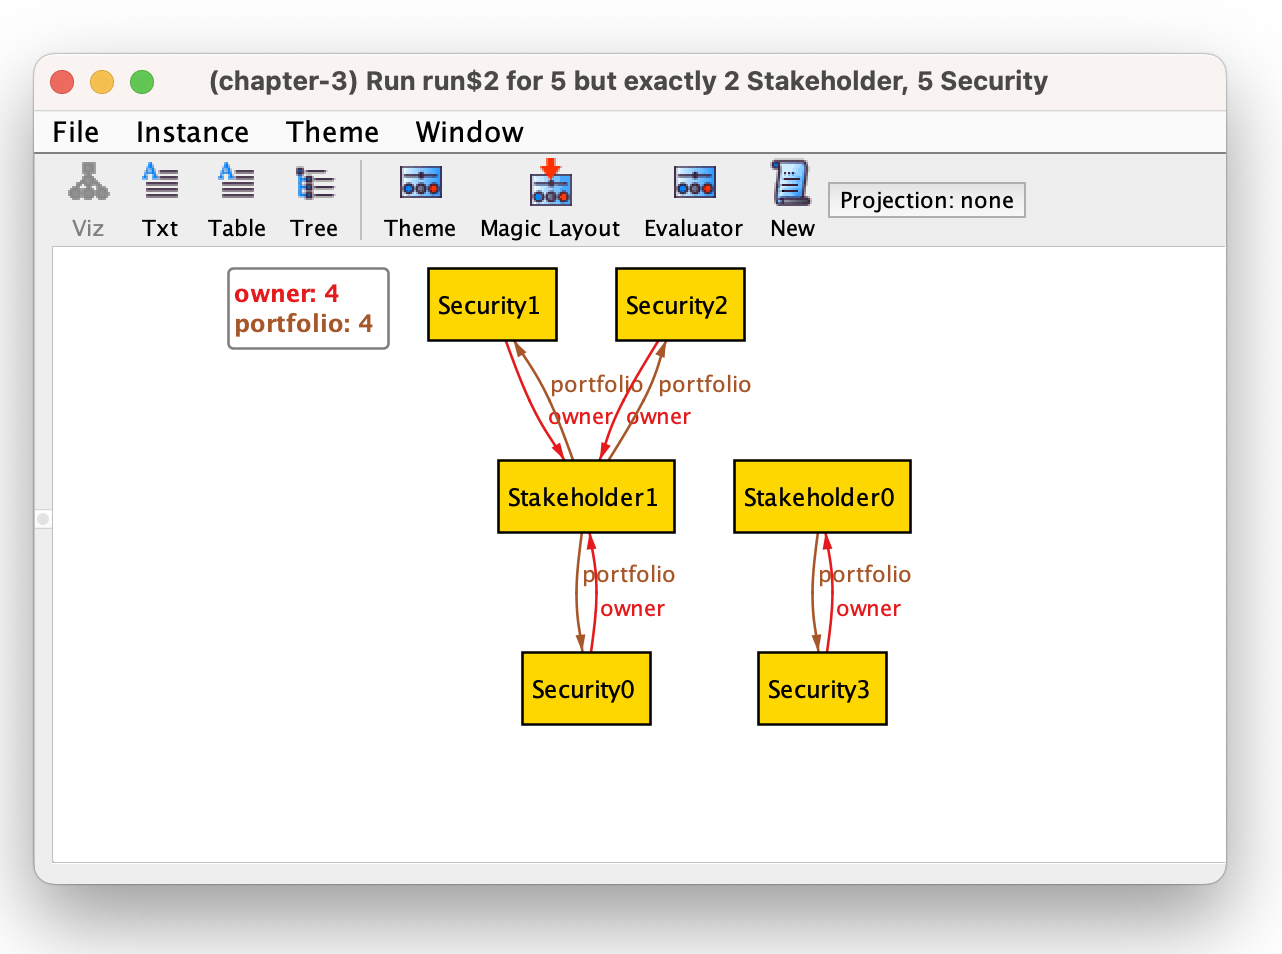
\includegraphics[width=0.8\textwidth]{images/alloy-run.png}}
	\caption{A sample instance generated by Alloy}\label{fig:alloy-run}
\end{figure}

\subsection{Refining a model}

We know the model is correct (up to a bound). But why? We can use Alloy to find out.

\newpage

The technique is to turn the \verb|invOwnerPort| fact into a \textit{predicate}; meaning that we do not assume it holds. But we can still ask Alloy to check whether it \textit{suffices} for \verb|noSharedOwnership| to hold, with a small change in the model:

\begin{listing}[H]\label{lst:alloy-strengthen}
	\begin{minted}{alloy}
pred invOwnerPort { ~owner = portfolio }
\end{minted}
	\caption{Strengthening the model}
\end{listing}

Now, the \verb|noSharedOwnership| assertion does not hold anymore, since we can find a counterexample:

\begin{listing}[H]\label{lst:alloy-strengthen-output}
	\begin{verbatim}
Executing "Check noSharedOwnership for 5"
Solver=minisatprover(jni) 
    Bitwidth=4 MaxSeq=5 
    SkolemDepth=4 Symmetry=20 Mode=batch
Generating CNF...
767 vars. 70 primary vars. 1177 clauses. 85ms.
Solving...
Counterexample found. Assertion is invalid. 14ms.
\end{verbatim}
	\caption{Alloy's output with a counterexample after strengthening the model}
\end{listing}

We call \verb|check| with a modified assertion, namely:

\begin{listing}[H]\label{lst:alloy-strengthen-check}
	\begin{minted}{alloy}
check noSharedOwnershipAlt {
    invOwnerPortfolio implies {
        no disj s1, s2 : Stakeholder | overlap
    }
}
\end{minted}
	\caption{Checking the model again, considering the strengthened assumptions}
\end{listing}

\newpage

Now we see that the model is still correct. That holds, but only because of the \verb|invOwnerPortfolio| predicate:

\begin{listing}[H]\label{lst:alloy-strengthen-check-output}
	\begin{verbatim}
Executing "Check noSharedOwnershipAlt"
Solver=minisatprover(jni) 
    Bitwidth=4 MaxSeq=4 
    SkolemDepth=4 Symmetry=20 Mode=batch
Generating CNF...
318 vars. 30 primary vars. 476 clauses. 104ms.
Solving...
No counterexample found. Assertion may be valid. 6ms.
core reduced from 8 to 6 top-level formulas. 23ms.
\end{verbatim}
	\caption{Alloy's output showing no counterexample after considering the strengthened assumptions}
\end{listing}

There is much going on underneath Alloy to make this possible, ultimately relying on the KodKod library~\cite{TorlakJackson2007} to translate Alloy problems to and from SAT problems.

A full presentation of Alloy is beyond the scope of this work, but can be found in the Software Abstractions book by Daniel Jackson~\cite{jackson-2012}.

\section{From JSON Schema to Alloy}

The OCF is chiefly a data format, while we are looking for a conceptual model. Nevertheless, the OCF is a good starting point for a conceptual model, and we can use it to derive a conceptual model that is more expressive and that can be used to validate capitalization tables.

The general approach has the following steps:

\begin{enumerate}
	\item Define the signatures roughly matching the documents in the JSON Schema, even if we must declare them as abstract before refining them
	\item Refine the signatures by adding fields and constraints, based on the keys and values in the JSON Schema
	\item Add expected properties (of the model) as assertions composed of predicates
	\item Check that assertions hold, or debug the model until they do
\end{enumerate}

Step 1 is very mechanical and straightforward. Step 2 requires some attention to detail, since relations in JSON schema are very different from those in Alloy. JSON Schema mostly defines JSON objects, which are associative maps. Some documents define an array of objects, or refer to other documents by ID.~On the other hand, Alloy provides fine-grained control over the arity and multiplicity of relations. Step 3 requires domain expertise and some training in the background relations, set and logic, and some creativity. Step 4 is a matter of running the Alloy Analyzer and checking the results, plus some debugging.

The whole process is not exceedingly difficult to perform, specially if compared to alternatives, Such as Z, TLA$^{+}$, or dependently typed languages and proof assistants such as Agda, Coq or Idris. It resembles writing SQL schemas or business domain entities in object-oriented languages, but it does require some familiarity with mathematics (set theory and logic).

\section{A brief overview of Alloy related literature}

Alloy is cited in more than 1,200 papers, with many extensions and applications
in software design and modeling. Alloy$\ast$ is a higher-order extension of
Alloy that can be used for program synthesis, since it supports higher-order
quantification~\cite{Milicevic2017}. $\alpha{Rb}y$ is an embedding of Alloy in
Ruby~\cite{Arby}.

A number of other modeling languages have been translated to or partially modeled in Alloy\cite{alloy-case-studies}, including UML, $i^\star$, CVL, Event-B and, Z, OCL.\@Alloy can also be used with verification languages such as ACL2 or Isabelle.

Alloy has been used in a wide range of applications in software engineering, database design, \gls{security} analysis~\cite{Carpio2021}\cite{Chen2006}, multiagent negotiations~\cite{Podorozhny}. It has also been applied to modeling beyond computer science, such as a model for central bank policy~\cite{Johnson2021}. A model of the same-origin-policy used in web browsers can be found in the 500 Lines or Less open-source book~\cite{500Lines19:online}.

\textit{We were unable to find previous models of \glspl{capitalization-table} in Alloy.}

\section{Consistency of Capitalization Tables - Alloy Model}
\label{ch:transaction-tracing}
\label{sec:transaction-tracing}

We developed an Alloy model based on the OCF that encompasses the OCF structure and the semantics of transactions permitted in financial systems.
In this section, we explore the portion of the Alloy model that ensures the consistency of \glspl{transaction} that affect capitalization tables. 

A \gls{capitalization-table} tracks the ownership stakes and capital structure of a company. The \glspl{transaction} that typically affect a \gls{capitalization-table} include \glspl{issuance}, cancellations, and transfers of  \glspl{security} 
%
(model overview in Fig.~\ref{fig:metamodel}).

\begin{figure}[!h]
	\centering
	\fbox{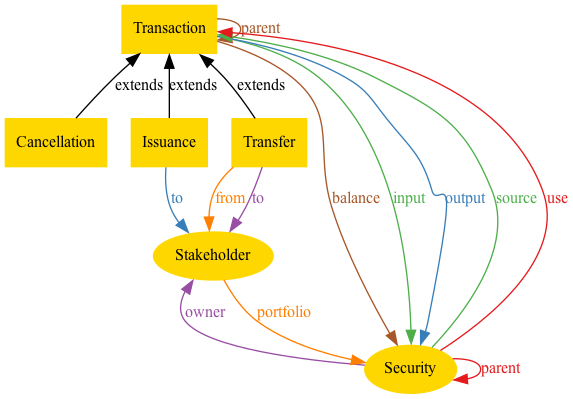
\includegraphics[width=0.7\textwidth]{images/metamodel5.png}}
	\caption{Transaction tracing metamodel: 
	Rendered by the Alloy Analyzer \label{fig:metamodel}}
\end{figure}

%\section{Introduction}

A \gls{capitalization-table} is built as new \glspl{transaction} are recorded. The Open Cap Table format proposes a ''transaction tracing model'' in which \glspl{security} are identified with unique identifiers and \glspl{transaction} refer to those identifiers when issuing, canceling, or transferring \glspl{security}.

The purpose of the transaction tracing model is to provide auditable \glspl{security} traceability. The Alloy model then needs to conform to the requirements for a consistent model for capitalization tables and enforce certain properties.

\subsection{Expected Properties}
\label{sec:exp-properties}

%Let's begin by defining the expected properties that the model must hold. 
The following properties must be satisfied regarding the graph of \glspl{security} and \glspl{transaction}:


\begin{description}
	\item [P1:] All \glspl{security} can be traced back to an Issuance.
	\item [P2:] All \glspl{transaction} can be traced back to an Issuance.
	\item [P3:] There can be no cycles in the \gls{security} hierarchy. This guarantees that every \gls{security} can be traced back to a root security.
	\item [P4:] There can be no cycles in the transaction hierarchy. This guarantees that every transaction can be traced back to a root transaction.
\end{description}

Additionally, the following accounting identity-related properties are defined:

\begin{description}
	\item [P5:] The number of shares in circulation should be less than or equal to the number of shares issued.
	\item [P6:] No \glspl{security} can have a negative number of shares.
	\item [P7:] The sum of shares in all portfolios should be equal to the number of shares issued minus the number of shares cancelled.
\end{description}

The properties above cannot be expressed in JSON Schema, but are expected for a consistent model of capitalization tables. The Alloy model must ensure that these properties hold, as checked by the Alloy Analyzer.

%We will give precise Alloy predicates for each of the properties.

\subsection{The Alloy Model}

This section presents the main elements of the model, illustrating each signature, predicate, and fact with a code excerpt.

\subsubsection{Securities and Transactions.}

The first elements consists of signatures for \glspl{security} and \glspl{transaction}, together with opening of the ordering and graph modules for both signatures, as they will form a complex structure that can be traced back to issuances (Listing \ref{list:security-transitions}).

\begin{listing}[!h]
 \begin{multicols}{2}
	\begin{minted}[fontsize=\footnotesize]
     {alloy}
open util/ordering[Security]
open util/ordering[Transaction]

open util/graph[Security]
open util/graph[Transaction]

sig Security {
    shares : Int,
    source : one Transaction,
    use : lone Transaction,
    parent : lone Security,
    owner : Stakeholder
} {
    nonneg[shares]
}

abstract sig Transaction {
    shares : Int,
    input : lone Security,
    output : lone Security,
    balance : lone Security,
    parent : lone Transaction
} {
    pos[shares]
}
fact {
    use = ~input
}
fact {
    source = ~(output + balance)
}
\end{minted}
\end{multicols}
	\caption{Security and Transaction Signatures and Constraints
    \label{list:security-transitions}
    }
\end{listing}

The \verb|Transaction| signature is given abstract because a \verb|Transaction| is never instantiated directly; they may have different types of \glspl{transaction}, such as issuances, cancellations, and transfers. Those types of \glspl{transaction} are defined afterwards.

Two constraints are stated as facts to relate the \verb|use| and \verb|source| fields of \glspl{security} to the \verb|input| and \verb|output| fields of \glspl{transaction}. The \verb|use| field of a \gls{security} is the transaction that uses the \gls{security} as input. The \verb|source| field of a \gls{security} is the transaction that uses the \gls{security} as output.
%
%\begin{listing}[!h]
% \begin{multicols}{2}
%	\begin{minted}[fontsize=\footnotesize]
%     {alloy}
%fact {
%    use = ~input
%}
%fact {
%    source = ~(output + balance)
%}
%\end{minted}
%\end{multicols}
%	\caption{Security Use and Source
%    \label{lst:tt-alloy-security-and-transaction-signatures}}
%\end{listing}
%
The \verb|~| operator to invert the binary relations is used for \verb|input| and \verb|output| because they denote the same relation with the opposite direction.

%The three transaction types are given below.

\subsubsection{Transaction types.}

We consider three types of transaction in the model because they subsume all other more specific types of transaction. Any transaction is a composition of creation and destruction of  \glspl{security}.  Transfers, in particular, are a combination of an issuance and a cancellation (Listing \ref{lst:tt-alloy-transaction-types}).

\begin{listing}[!h]
 \begin{multicols}{2}
	\begin{minted}[fontsize=\footnotesize]
     {alloy}
sig Issuance extends Transaction {
    to : Stakeholder
} {
    no input
    no balance
    one output
    no (Transaction <: parent)
}
sig Cancellation extends Transaction {} {
    no output
    lone balance
    one input
    one (Transaction <: parent)
}
sig Transfer extends Transaction {
    from : Stakeholder,
    to : Stakeholder - from
} {
    one input
    one output
    lone balance
    one (Transaction <: parent)
}
\end{minted}
\end{multicols}
	\caption{Transaction Types}
\label{lst:tt-alloy-transaction-types}
\end{listing}

All \glspl{transaction} have \verb|parent|, \verb|input|, \verb|output|, and \verb|balance| fields, but each transaction uses only a subset of them. Additional fields, appearing after the signature, constraint the \glspl{transaction}.
%
For instance, the \verb|Issuance| transaction has a \verb|to| field stating who will own the issued security, while the \verb|Transfer| transaction has \verb|from| and \verb|to| fields stating who will transfer the \gls{security} from and to.

\subsubsection{Issuance constraints.}

The behavior of the Issuance is encoded in a single fact (Listing \ref{lst:tt-alloy-issuance-constraints}). The first line equates the number of shares of the newly issued \gls{security} to the number of the shares in the issuance, while the following lines bind other specific fields to their appropriate values.

\begin{listing}[!h]
 \begin{multicols}{2}
	\begin{minted}[fontsize=\footnotesize]
     {alloy}
fact {
    all iss : Issuance {
        eq[iss.output.shares, iss.shares]
        iss.output.source = iss
        iss.output.owner = iss.to
        iss.output in iss.to.portfolio
    }
}
\end{minted}
\end{multicols}
	\caption{Issuance Constraints}
\label{lst:tt-alloy-issuance-constraints}
\end{listing}


\subsubsection{Cancellation constraints.}

%The case for a cancellation is more complex because it must distinguish between partial and complete cancellations. This is done by comparing the number of shares in the cancellation and in the cancelled security, and giving different constraints for each case.
%%
%It is encoded in a single fact (Listing \ref{lst:tt-alloy-cancellation-constraints}).

\begin{listing}[!h]
% \begin{multicols}{2}
	\begin{minted}[fontsize=\footnotesize]
     {alloy}
fact {
    all can : Cancellation {
        lt[can.shares, can.input.shares] implies {
            // In this case, the transaction is partial.
            can.input.use = can
            can.balance.source = can
            eq[can.balance.shares, sub[can.input.shares, can.shares]]
            lt[can.input, can.balance]
            can.balance.owner = can.input.owner
            can.balance in can.input.owner.portfolio
            can.balance.parent = can.input
            can.parent = can.input.source
        } else {
            can.input.use = can
            eq[can.input.shares, can.shares]
            can.parent = can.input.source
            no can.balance            
        }
    }
}
\end{minted}
%\end{multicols}
	\caption{Cancellation Constraints}
\label{lst:tt-alloy-cancellation-constraints}
\end{listing}

The case for a cancellation is more complex because it must distinguish between partial and complete cancellations. This is done by comparing the number of shares in the cancellation and in the cancelled security, and giving different constraints for each case.
%
It is encoded in a fact (Listing \ref{lst:tt-alloy-cancellation-constraints}).

The constraints are now more detailed to ensure the balancing of shares, and the fields used to relate \glspl{security} and \glspl{transaction} in a graph.% (the \verb|parent| field, ultimately).

\subsubsection{Transfer constraints.}

Here no new logic needs to be introduced, but we now use all three fields (\verb|input|, \verb|output|, and \verb|balance|) if a partial transfer is performed (Listing \ref{lst:alloy-transfer-constraints}). %It is unfortunately more verbose.

\begin{listing}[!h]
% \begin{multicols}{2}
	\begin{minted}[fontsize=\footnotesize]
     {alloy}
fact {
    all xfer : Transfer {
        lt[xfer.shares, xfer.input.shares] implies {
            // In this case, the transaction is partial.
            xfer.input.use = xfer
            xfer.output.source = xfer
            xfer.balance.source = xfer
            eq[xfer.output.shares, xfer.shares]
            eq[xfer.balance.shares, sub[xfer.input.shares, xfer.shares]]
            lt[xfer.input, xfer.output]
            lt[xfer.input, xfer.balance]
            xfer.output.owner = xfer.to
            xfer.input.owner = xfer.from
            xfer.balance.owner = xfer.from
            xfer.from.portfolio = xfer.from.portfolio + xfer.balance
            xfer.to.portfolio = xfer.to.portfolio + xfer.output
            xfer.output.parent = xfer.input
            xfer.balance.parent = xfer.input
        } else {
            xfer.input.use = xfer
            xfer.output.source = xfer
            eq[xfer.output.shares, xfer.shares]
            eq[xfer.shares, xfer.input.shares]
            lt[xfer.input, xfer.output]
            xfer.output.owner = xfer.to
            xfer.input.owner = xfer.from            
            xfer.to.portfolio = xfer.to.portfolio + xfer.output
            xfer.output.parent = xfer.input
            no xfer.balance
        }
    }
}
\end{minted}
%\end{multicols}
	\caption{Transfer Constraints
             \label{lst:alloy-transfer-constraints}
             }
\end{listing}

We observe that the required bookkeeping in a structural Alloy model can become complex. As we add more constraints to our model, we can rely on the Alloy Analyzer to ensure that it remains consistent.

\subsection{Model Properties}

%\subsubsection{Ordering of Transaction and securities}

The hypothesis for proving the properties of the system  will be based on the ordering provided by the \verb|ordering| module for \glspl{transaction} and \glspl{security} (Listing \ref{lst:tt-alloy-ordering}). In the ordering, there is a consistent pattern for parents to always come before their children. Other auxiliary functions are defined in Appendix \ref{app:aux-functions}.


\begin{listing}[!h]
 \begin{multicols}{2}
	\begin{minted}[fontsize=\footnotesize]
     {alloy}
pred orderingOfSecurities {
    all sec : Security {
        some sec.parent implies {
            lt[sec.parent, sec]
        }
    }
}
pred orderingOfTransactions {
    all tx : Transaction {
        some tx.parent implies {
            lt[tx.parent, tx]
        }
    }
}
\end{minted}
\end{multicols}
	\caption{Ordering of Securities and \glspl{transaction}}
\label{lst:tt-alloy-ordering}
\end{listing}

\subsubsection{Properties.}

The properties described in this section are the expected features that are required to provide consistency in cap tables during transaction updates, as previously defined in Section \ref{sec:exp-properties}.
%
The first property states that if the \glspl{security} are ordered, then the graph of \glspl{security} forms a forest (Listing \ref{lst:tt-alloy-properties-graph-securities}). A forest is a collection of trees, which is a stronger condition than merely being a directed acyclic graph. Similarly, a property for \glspl{transaction} is defined.

\begin{listing}[!h]
	\begin{minted}[fontsize=\footnotesize]{alloy}
check {
    orderingOfSecurities => forest[~(Security <: parent)]
}
check {
    orderingOfTransactions => forest[~(Transaction <: parent)]
}
\end{minted}
	\caption{Forest of Securities and Transactions}
\label{lst:tt-alloy-properties-graph-securities}
\label{lst:tt-alloy-properties-graph-transactions}
\end{listing}

%And a similar property for \glspl{transaction}.
%
%\begin{listing}
%	\begin{minted}{alloy}
%check {
%    orderingOfTransactions => forest[~(Transaction <: parent)]
%}
%\end{minted}
%	\caption{Forest of \glspl{transaction}}
%\label{lst:tt-alloy-properties-graph-transactions}
%\end{listing}

%\textbf
{These properties cannot be modelled in JSON Schema, since we need to compare values in two different documents (in JSON Schema parlance).} But they can be clearly expressed in Alloy.

In Listing \ref{lst:tt-alloy-properties-accounting}, accounting identities in the spirit of the given in the start of the chapter are simply to state: 
\todo[inline]{texto vago...aqui é preciso relacionar essas props com as propriedades no início da seção... pra mostrar o que foi possível definir facilmente, e o poder do novo modelo. Essa é a seção mais importante! Numerei as props para poder relacionar com essa seção.}

\begin{listing}[!h]
	\begin{minted}[fontsize=\footnotesize]{alloy}
cancelledSharesAlwaysLessThanIssued : check {
    lte[cancelledShares, issuedShares]
} for 3
nonNegativityOfIssuedShares : check {
    nonneg[issuedShares]
} for 3
nonNegativityOfCancelledShares : check {
    nonneg[cancelledShares]
} for 3
aliveLessThanIssued : check {
    lte[aliveShares, issuedShares]
} for 3
\end{minted}
	\caption{Accounting Identities}
\label{lst:tt-alloy-properties-accounting}
\end{listing}

Another important property for all those financial systems regards investor portfolios: they must all be disjoint (Listing \ref{lst:tt-alloy-properties-disjoint-portfolios}).

\begin{listing}[!h]
	\begin{minted}[fontsize=\footnotesize]{alloy}
check {
    all o1, o2 : Stakeholder {
        some o1.portfolio & o2.portfolio implies o1 = o2
    }
}
\end{minted}
	\caption{Disjoint Portfolios}
\label{lst:tt-alloy-properties-disjoint-portfolios}
\end{listing}

And we close by checking that all floating shares are owned. 
\todo[inline]{texto vago. o que isso significa na prática, ou em relação às propriedades do início da seção??}

\begin{listing}[!h]
	\begin{minted}[fontsize=\footnotesize]{alloy}
fun portfolioShares[stakeholder : Stakeholder] : Int {
    sum sec : stakeholder.portfolio | 
             (sec in aliveSecurities implies sec.shares else 0)
}
fun portfolioSharesAll : Int {
    sum stakeholder : Stakeholder | portfolioShares[stakeholder]
}
check {
    eq[aliveShares, portfolioSharesAll]
}
\end{minted}
	\caption{Floating Shares}
\label{lst:tt-alloy-properties-floating-shares}
\end{listing}

\section{An example with a long chain of transactions}

\todo[inline]{aqui precisamos contar uma estória sobre as transações reais e como esse recurso mostraria o que acontece com o modelo. }

To give an interesting example, we use the \verb|depth| function we defined and asked Alloy to find a ``long'' instance. 
%
Figure~\ref{fig:tt-alloy-example-transaction-single-issuance} shows the result of running the example. 

\begin{listing}[!h]
	\begin{minted}[fontsize=\footnotesize]{alloy}
run {
    some sec : Security | depth[sec] > 3
} for 5
\end{minted}
	\caption{Example}
\label{lst:tt-alloy-example}
\end{listing}


\begin{figure}[!h]
	\centering
	\fbox{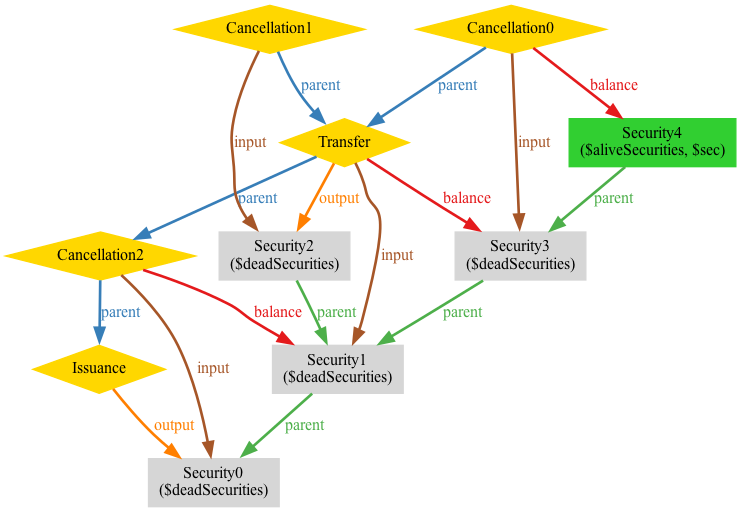
\includegraphics[width=0.9\textwidth]{images/spine.png}}
	\caption{A long chain of \glspl{transaction} arising from a single issuance}\label{fig:tt-alloy-example-transaction-single-issuance}
\end{figure}

In this instance, a security, denoted as \verb|Security$0|, was initially issued and subsequently partially cancelled. This cancellation resulted in the creation of a new security, referred to as \verb|Security$1|, which represents the remaining balance. Furthermore, a partial transfer of \verb|Security$1| led to the generation of two distinct securities, namely \verb|Security$3| and \verb|Security$4|, serving as the output and balance, respectively. Securities \verb|Security$2| and \verb|Security$3| are subsequently cancelled, while \verb|Security$4| is established as the balance \gls{security} to compensate for the cancellation of \verb|Security$3|.



\todo[inline]{é preciso enfatizar: como as instâncias criadas auxiliam o negócio (sturtups); que existem outras instâncias; e como a instância gerada satisfaz as propriedades, mantendo a consistência das cap-tables}

\section{Conclusion}

Alloy has been used in a wide range of applications in software engineering, database design, \gls{security} analysis~\cite{Carpio2021}\cite{Chen2006}, multiagent negotiations~\cite{Podorozhny}. It has also been applied to modeling beyond computer science, such as a model for central bank policy~\cite{Johnson2021}. A model of the same-origin-policy used in web browsers can be found in the 500 Lines or Less open-source book~\cite{500Lines19:online}.
%
There is a lack of existing models of \glspl{capitalization-table} in Alloy, as well as an absence of semantic models for this particular domain.

By using Alloy, we have been able to model the \gls{capitalization-table} of a company, and to show how a long chain of \glspl{transaction} could be rigorously modeled in a verifiable, auditable manner, in a way that was not possible within the original JSON Schema implementation.
%
We started with a \textit{data} specification and worked towards a \textit{domain} specification. The syntactical nature of the original \textit{data} model was enriched with a \textit{semantic} nature of the \textit{domain} behavior, taking into account the relationships between various types of entities and expected invariants (based on domain knowledge).

As a result, in the transaction tracing system we could:

\begin{itemize}
	\item uncover an interesting symmetry between the graphs of \glspl{transaction} and \glspl{security} in the transaction tracing model, and used that data structure to ensure that all \glspl{security} and transactions in the model are auditable.
	\item enforce constraints on the \glspl{transaction} and the \glspl{security} and ensured that basic accounting identities are respected.
\end{itemize}

The semantics of the rules in legal documents, which might be ambiguous due to the natural language used, can be made explicit in a formal model. This is a first step towards a more general formalization of business contract rules, which can be used to reason about the rules, and to verify that the rules are implemented correctly in software systems.

The model already incorporates additional knowledge domain aspects by specifying the logical components of Vesting and Convertible Securities. Although the existing components of capitalization tables offer a coherent model, our goal is to enhance the model by incorporating temporal features. In addition to this, our current research focuses on exploring the potential usage of the Alloy application programming interface (API) for the purpose of extracting source code from the Alloy models. This approach would make easier the production of business contract implementations based on an established model.


%%\chapter{A model for enhancing the expressiveness of vesting rules}\label{ch:vesting-system}

In this chapter, we will walk through the Alloy model, which enhances upon an open-source JSON Schema model. We incorporate and demonstrate the use of And/Or/Not operators, thus extending the triggers to more of a domain-specific language that supports propositional logic. In particular, we leverage the not operator with the ExactDate trigger to express the ``until condition'', which allows the model to express contract clauses that stipulate a milestone to be achieved until a given date.

The model is shown in Figure~\ref{fig:vs-metamodel}.
\begin{figure}[H]
	\centering
	\fbox{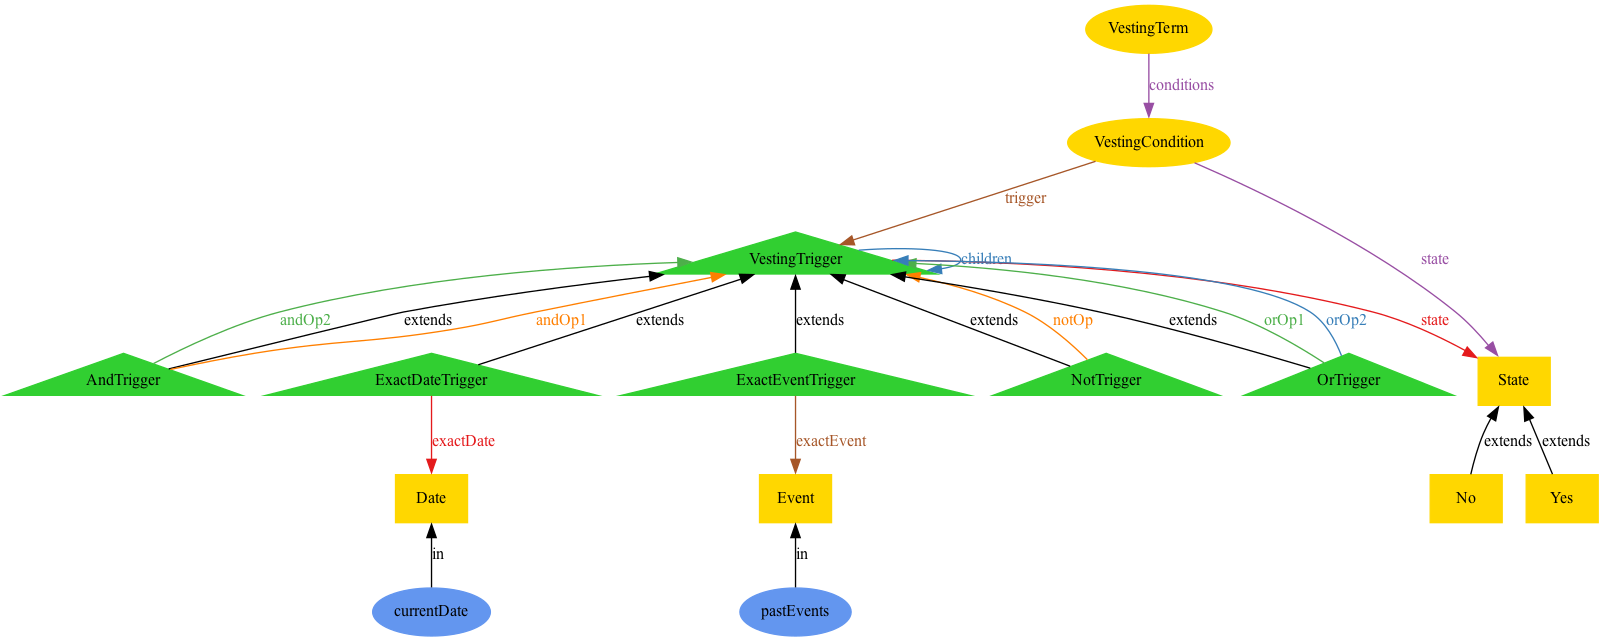
\includegraphics[width=\textwidth]{images/metamodel4.png}}
	\caption{Vesting system metamodel}\label{fig:vs-metamodel}
	As rendered by the Alloy Analyzer
\end{figure}

\section{Vesting Terms and Conditions}

Our Alloy model begins with the definition of the \verb|VestingTerm|, \verb|VestingCondition| and \verb|VestingTrigger| signatures.

A \verb|VestingTerm| represents a set of conditions that need to be met and the authorized shares for the vesting term. The \verb|VestingCondition| signifies a particular condition or a trigger.

Since our modeling has no form of mutation involved, there is no need to identify a vesting term with a vesting condition \textemdash{whether other vesting terms refer to the same conditions is harmless, as long as the authorized shares match the shares in the conditions}.

\begin{listing}[H]\label{listing:vs:vesting-term}
	\begin{minted}{alloy}
	sig VestingTerm {
		conditions : set VestingCondition,
		authorizedShares : Int
	}
	\end{minted}
	\caption{Vesting term signature}
\end{listing}

\begin{listing}[H]\label{fig:vs:vesting-condition}
	\begin{minted}{alloy}
sig VestingCondition {
    trigger : VestingTrigger,
    state : State,
    shares : Int
}
\end{minted}
	\caption{Vesting condition signature}
\end{listing}

This fact relating shares in vesting terms and shares in vesting conditions is not expressible in JSON Schema because it is a constraint that relates two different entities and evaluates arithmetic.

\begin{listing}[H]\label{fig:vs:fact-vesting-condition}
	\begin{minted}{alloy}
fact {
    all t : VestingTerm {
        lte[sum[t.conditions.shares], t.authorizedShares]
    }
}
\end{minted}
	\caption{Fact\textemdash{Only as many shares as authorized can be granted}}
\end{listing}

\section{Vesting Triggers}

\verb|VestingTrigger| is an abstract sig that signifies the state and its children.

\begin{listing}[H]\label{fig:vs:trigger}
	\begin{minted}{alloy}
abstract sig VestingTrigger {
    state : State,
    children : set VestingTrigger
}
\end{minted}
	\caption{The abstract Vesting trigger signature}
\end{listing}

It has four extensions: \verb|ExactDateTrigger|, \verb|ExactEventTrigger|, \verb|AndTrigger|, and \verb|OrTrigger|. \verb|ExactDateTrigger| and \verb|ExactEventTrigger| trigger on an exact date and event, respectively.

\begin{listing}[H]\label{fig:vs:exact-date-trigger}
	\begin{minted}{alloy}
sig ExactDateTrigger extends VestingTrigger {
    exactDate : one Date
} {
    no children
}
\end{minted}
	\caption{Exact date trigger signature}
\end{listing}

\begin{listing}[H]\label{fig:vs:exact-event-trigger}
	\begin{minted}{alloy}
sig ExactEventTrigger extends VestingTrigger {
    exactEvent : one Event
} { 
    no children
}
\end{minted}
	\caption{Exact event trigger signature}
\end{listing}

\verb|AndTrigger| and \verb|OrTrigger| represent the logical AND and OR operations, where the trigger is computed from two other triggers. We further enhance this model by introducing a \verb|NotTrigger|, representing the logical NOT operation.

\begin{listing}[H]\label{fig:vs:and=trigger}
	\begin{minted}{alloy}
sig AndTrigger extends VestingTrigger {
	andOp1 : one VestingTrigger,
	andOp2 : one VestingTrigger - andOp1
} {
	children = andOp1 + andOp2
}
\end{minted}
	\caption{And trigger signature}
\end{listing}

\begin{listing}[H]\label{fig:vs:or-trigger}
	\begin{minted}{alloy}
sig OrTrigger extends VestingTrigger {
    orOp1 : one VestingTrigger,
    orOp2 : one VestingTrigger - orOp1
} {
	children = orOp1 + orOp2
}
\end{minted}
	\caption{Or trigger signature}
\end{listing}

\begin{listing}[H]\label{fig:vs:not-trigger}
	\begin{minted}{alloy}
sig NotTrigger extends VestingTrigger {
    notOp : one VestingTrigger
} {
    children = notOp
}
\end{minted}
	\caption{Not trigger signature}
\end{listing}

\textbf{This is a valuable contribution because it adds a propositional logic layer over the vesting rules in the original model}.


\section{Facts}

Facts establish the truth in our Alloy model. We define facts for \verb|ExactDateTrigger|, \verb|ExactEventTrigger|, \verb|AndTrigger|, \verb|OrTrigger| and \verb|NotTrigger| where we set their state based on the conditions of their triggers~\textemdash{this is how we give the evaluation rules for the vesting triggers}.

\subsection{Evaluation for dates and events}

\begin{listing}[H]\label{list:vs:fact-exact-date-trigger-eval}
	\begin{minted}{alloy}
fact {
	all t : ExactDateTrigger {
		lte[t.exactDate, currentDate] iff t.state = Yes
	}
}
\end{minted}
	\caption{Fact\textemdash{Exact date trigger evaluation}}
\end{listing}

\begin{listing}[H]\label{fig:vs:fact-exact-event-trigger-eval}
	\begin{minted}{alloy}
fact {
	all t : ExactEventTrigger {
		t.exactEvent in pastEvents iff t.state = Yes
	}
}
\end{minted}
	\caption{Fact\textemdash{Exact event trigger evaluation}}
\end{listing}

\subsection{Evaluation for And/Or/Not Triggers}

\begin{listing}[H]\label{fig:vs:fact-and-trigger-eval}
	\begin{minted}{alloy}
fact {
	all t : AndTrigger {
		t.state = Yes iff (t.andOp1.state = Yes and t.andOp2.state = Yes)
	}
}
\end{minted}
	\caption{Fact\textemdash{And trigger evaluation}}
\end{listing}

\begin{listing}[H]\label{fig:vs:fact-or-trigger-eval}
	\begin{minted}{alloy}
fact {
	all t : OrTrigger {
		t.state = Yes iff (t.orOp1.state = Yes or t.orOp2.state = Yes)
	}
}
\end{minted}
	\caption{Fact\textemdash{Or trigger evaluation}}
\end{listing}

\begin{listing}[H]\label{fig:vs:fact-not-trigger-eval}
	\begin{minted}{alloy}
fact {
    all t : NotTrigger {
        t.state = Yes iff t.notOp.state = No
    }
}
\end{minted}
	\caption{Fact\textemdash{Not trigger evaluation}}
\end{listing}

\section{Functions and Checks}

We now introduce several functions to calculate vested and granted shares. The function \verb|vestedShares| returns the number of vested shares, and \verb|grantedShares| returns the number of granted shares for a vesting term. We also introduce checks to ensure that granted shares are greater than or equal to vested shares and that they are positive, and that vested shares are non-negative.

\begin{listing}[H]\label{fig:vs:fun-vested-shares}
	\begin{minted}{alloy}
fun vestedShares[c : VestingCondition] : Int {
    c.state = Yes implies c.shares else 0
}

fun vestedShares[t : VestingTerm] : Int {
    sum c : t.conditions | vestedShares[c]
}
\end{minted}
	\caption{Functions\textemdash{Vested shares}}
\end{listing}

\begin{listing}[H]\label{fig:vs:fun-granted-shares}
	\begin{minted}{alloy}
fun grantedShares[t : VestingTerm] : Int {
    sum c : t.conditions | c.shares
}
\end{minted}
	\caption{Functions\textemdash{Granted shares}}
\end{listing}

\begin{listing}[H]\label{fig:vs:check-granted-shares-gte-vested-shares}
	\begin{minted}{alloy}
check {
    all t : VestingTerm {
        gte[grantedShares[t], vestedShares[t]]
    }  
}

fact {
    all t : VestingTerm {
        lte[sum[t.conditions.shares], t.authorizedShares]
    }
}

check {
    all t : VestingTerm {
        pos[grantedShares[t]]
    }  
}

check {
    all t : VestingTerm {
        nonneg[vestedShares[t]]
    }  
}
\end{minted}
	\caption{Checks\textemdash{Granted shares greater than or equal to vested shares}}
\end{listing}

This modeling approach enables linking to a model very similar to the transaction tracing model by adding \glspl{transaction} similar to \glspl{exercise} that output a new plan \gls{security} with more exercised shares and the same vesting term.

\section{Conclusion}

We improved the semantics of the original model as we translated it to Alloy. Our improvement came out of identifying the space for a propositional logic layer over the original model. We closed the chapter by showing how an instance from our model, when expressed in prose in legal documents, is difficult to understand and analyze.

%%\chapter{Case study}\label{ch:contract}

We should now show a translation of a legal contract to an instance of our model. 

The translation is done by programming a predicate that selects instances which match an expert's understanding of the contract. The process is not at all automatic, although the constraints added to the problem do prevent programming errors.

Our particular case will be a typical Employee Stock Option Program (ESOP) contract. Those are both common and costly to operate, since they depend on all models we presented in~\ref{ch:transaction-tracing} and~\ref{ch:vesting-system}, and can involve hundreds of employees. They are both complex and large.

\section{Employee Stock Option Programs}

\Glspl{startup-company} award stock options to employees as part of their compensation. Stock options are only valuable if the underlying stock exceeds a certain price, so this form of incentive corresponds to the defining property of \glspl{startup-company}, which is to start small and grow extremely fast.

Since they are complex contracts and issued in large numbers, they are an adequate test for our model. They depend on the invariants that we introduced in our models, which were only possible with a more powerful modeling language.

\section{Characterizing an instance via a predicate}

We can ask Alloy to find an instance for a vesting term with triggers in both Yes and No states, including use of our new operators.

\begin{listing}[H]\label{fig:vs:run-vesting-term}
	\begin{minted}{alloy}
run { 
    Yes + No = ExactDateTrigger.state
    Yes + No = ExactEventTrigger.state
    some AndTrigger
    some OrTrigger
    one VestingTerm
} for 6
\end{minted}
	\caption{Run\textemdash{Vesting term}}
\end{listing}

\section{Visualizing the instance}

From the instance, we can use the Alloy visualizer to find the following picture:

\textbf{{PLACEHOLDER}}

\section{A natural language, prose rendering of the instance}

\subsection{issuance}

The issuance has a simple wording, and the variation is in how the number and cost of shares and the price per share are expressed. Given two, the third is defined.

\begin{multicols}{2}
	\begin{figure}[H]\label{fig:doc-tt-issuance}
		\centering
		\begin{minipage}{0.4\textwidth}
			\textbf{Share Investment Agreement}
			\\
			Hereby, the Investor agrees to invest in the Company the amount of 1,000 USD, in exchange for 20\% shares of the Company's stock.
		\end{minipage}
	\end{figure}
	\columnbreak{}
	\begin{figure}[H]\label{fig:doc-tt-issuance-2}
		\centering
		\begin{minipage}{0.4\textwidth}
			\textbf{Share Investment Agreement}
			\\ \@
			Hereby, the Investor agrees to purchase 1,000\@shares of the Company's stock, at the price per share of USD 1.
		\end{minipage}
	\end{figure}
\end{multicols}

More complication is possible if \glspl{transaction} refer to past prices:

\begin{multicols}{2}
	\begin{figure}[H]\label{fig:doc-tt-issuance-3}
		\centering
		\begin{minipage}{0.4\textwidth}
			\textbf{Share Investment Agreement}
			\\
			Hereby, the Investor agrees to invest in the Company in the amount of 1,000 USD, at 2 times the price per share paid by the Investor in the previous round.
		\end{minipage}
	\end{figure}
	\columnbreak{}
	\begin{figure}[H]\label{fig:doc-tt-issuance-4}
		\centering
		\begin{minipage}{0.4\textwidth}
			\textbf{Share Investment Agreement}
			\\
			Hereby, the Investor agrees to purchase 1,000 shares of the Company's stock, at a 20\% discount from the price paid by the Investor in the previous round.
		\end{minipage}
	\end{figure}
\end{multicols}

\subsection{Cancellation}

The cancellation is also simple, and the variation is in how the number of shares is expressed.

\begin{multicols}{2}
	\begin{figure}[H]\label{fig:doc-tt-cancellation}
		\centering
		\begin{minipage}{0.4\textwidth}
			\textbf{Share Cancellation Agreement}
			\\
			Hereby the Company cancels 50\% of the stocks held by the Investor signed below.
		\end{minipage}
	\end{figure}
	\columnbreak{}
	\begin{figure}[H]\label{fig:doc-tt-cancellation-2}
		\centering
		\begin{minipage}{0.4\textwidth}
			\textbf{Share Cancellation Agreement}
			\\
			Hereby the Company cancels 500 stocks held by the Investor signed below.
		\end{minipage}
	\end{figure}
\end{multicols}

\subsection{Transfer}

The transfer is also simple, and the variation is in how the number of shares is expressed, and a receiving \gls{stakeholder} must also be defined:

\begin{multicols}{2}
	\begin{figure}[H]\label{fig:doc-tt-transfer}
		\centering
		\begin{minipage}{0.4\textwidth}
			\textbf{Share Transfer Agreement}
			\\
			Hereby, the Investor signed below transfers 50\% of the stocks held to the Investor signed below.
		\end{minipage}
	\end{figure}
	\columnbreak{}
	\begin{figure}[H]\label{fig:doc-tt-transfer-2}
		\centering
		\begin{minipage}{0.4\textwidth}
			\textbf{Share Transfer Agreement}
			\\
			Hereby, the Investor signed below transfers 500 stocks held to the Investor signed below.
		\end{minipage}
	\end{figure}
\end{multicols}

We have found examples that are typical of the difficulties in managing \glspl{capitalization-table} in spreadsheets or with no standards of any kind:

If a transaction states the number of shares as a percentage, the number of shares must be calculated from the total number of shares issued, and this requires tracing back the chain of \glspl{transaction} and  \glspl{security}.  If \glspl{transaction} refer to past prices or quantities, we also need to trace back the chain of transactions and \glspl{security} to find the relevant information.

This contract, in legal representation, would also have an unwieldy representation. That is why we need better formats and models for vesting systems: even the most basic vesting schedules are difficult to understand and represent.

\begin{figure}[H]\label{fig:vs:contract}
	\begin{minipage}{\linewidth}
		This Stock Grant Contract (hereinafter referred to as the ``Contract'') is entered into and effective as of the second agreed-upon date (the ``Effective Date'').

		\section*{Terms and Conditions}

		1. The parties to this Contract are the granter (the ``Granter'') and the grantee (the ``Grantee'').
		2. The Granter hereby grants the Grantee 7 authorized shares (the ``Shares'') of the Granter's stock, subject to the terms and conditions set forth herein.

		\subsection*{Vesting Schedule}

		1. First Condition: One share shall vest upon the simultaneous occurrence of the company reaching sales of USD 100M before the date promised to investors and another unspecified event, provided the state of affairs remains as originally agreed upon.
		2. Second Condition: One share shall vest on the fifth agreed-upon date, assuming the state of affairs remains as initially agreed upon.
		3. Third Condition: One share shall vest on the second agreed-upon date, given that the state of affairs has changed to the alternative agreed-upon state.
		4. Fourth Condition: One share shall vest upon the occurrence of the company reaching sales of USD 100M before the date promised to investors, provided the state of affairs remains as initially agreed upon.
		5. Fifth Condition: One share shall vest upon the occurrence of a second significant financial milestone, given that the state of affairs has changed to the alternative agreed-upon state.
		6. Sixth Condition: Two shares shall vest upon the occurrence of either the fifth agreed-upon date or the simultaneous occurrence of the company reaching sales of USD 100M before the date promised to investors and another unspecified event, provided the state of affairs remains as initially agreed upon.

		\subsection*{Miscellaneous}

		This Contract and all rights and obligations hereunder shall be binding upon and inure to the benefit of the parties hereto and their respective heirs, successors, and assigns. This Contract may not be assigned by either party without the prior written consent of the other party. This Contract shall be governed by and construed in accordance with the laws of the jurisdiction where the Granter is located.
	\end{minipage}
	\caption{Vesting Term Contract}
\end{figure}

\section{Discussion}

In practice, this means going over tens of legal documents and searching for the exact information needed. This is the problem that prompted the author into this field.
%%\input{sec-conclusion}

% ---- Bibliography ----
%
% BibTeX users should specify bibliography style 'splncs04'.
% References will then be sorted and formatted in the correct style.
%
%\bibliographystyle{splncs04}
%\bibliography{references}
%

%%------------------------------------------------------
%\section{First Section}
%\subsection{A Subsection Sample}
%Please note that the first paragraph of a section or subsection is
%not indented. The first paragraph that follows a table, figure,
%equation etc. does not need an indent, either.
%
%Subsequent paragraphs, however, are indented.
%
%\subsubsection{Sample Heading (Third Level)} Only two levels of
%headings should be numbered. Lower level headings remain unnumbered;
%they are formatted as run-in headings.
%
%\paragraph{Sample Heading (Fourth Level)}
%The contribution should contain no more than four levels of
%headings. Table~\ref{tab1} gives a summary of all heading levels.
%
%\begin{table}
%\caption{Table captions should be placed above the
%tables.}\label{tab1}
%\begin{tabular}{|l|l|l|}
%\hline
%Heading level &  Example & Font size and style\\
%\hline
%Title (centered) &  {\Large\bfseries Lecture Notes} & 14 point, bold\\
%1st-level heading &  {\large\bfseries 1 Introduction} & 12 point, bold\\
%2nd-level heading & {\bfseries 2.1 Printing Area} & 10 point, bold\\
%3rd-level heading & {\bfseries Run-in Heading in Bold.} Text follows & 10 point, bold\\
%4th-level heading & {\itshape Lowest Level Heading.} Text follows & 10 point, italic\\
%\hline
%\end{tabular}
%\end{table}
%
%
%\noindent Displayed equations are centered and set on a separate
%line.
%\begin{equation}
%x + y = z
%\end{equation}
%Please try to avoid rasterized images for line-art diagrams and
%schemas. Whenever possible, use vector graphics instead (see
%Fig.~\ref{fig1}).
%
%\begin{figure}
%\includegraphics[width=\textwidth]{fig1.eps}
%\caption{A figure caption is always placed below the illustration.
%Please note that short captions are centered, while long ones are
%justified by the macro package automatically.} \label{fig1}
%\end{figure}
%
%\begin{theorem}
%This is a sample theorem. The run-in heading is set in bold, while
%the following text appears in italics. Definitions, lemmas,
%propositions, and corollaries are styled the same way.
%\end{theorem}
%%
%% the environments 'definition', 'lemma', 'proposition', 'corollary',
%% 'remark', and 'example' are defined in the LLNCS documentclass as well.
%%
%\begin{proof}
%Proofs, examples, and remarks have the initial word in italics,
%while the following text appears in normal font.
%\end{proof}
%For citations of references, we prefer the use of square brackets
%and consecutive numbers. Citations using labels or the author/year
%convention are also acceptable. The following bibliography provides
%a sample reference list with entries for journal
%articles~\cite{ref_article1}, an LNCS chapter~\cite{ref_lncs1}, a
%book~\cite{ref_book1}, proceedings without editors~\cite{ref_proc1},
%and a homepage~\cite{ref_url1}. Multiple citations are grouped
%\cite{ref_article1,ref_lncs1,ref_book1},
%\cite{ref_article1,ref_book1,ref_proc1,ref_url1}.
%
%\subsubsection{Acknowledgements} Please place your acknowledgments at
%the end of the paper, preceded by an unnumbered run-in heading (i.e.
%3rd-level heading).
%
%%
%% ---- Bibliography ----
%%
%% BibTeX users should specify bibliography style 'splncs04'.
%% References will then be sorted and formatted in the correct style.
%%
%% \bibliographystyle{splncs04}
%% \bibliography{mybibliography}
%%
%\begin{thebibliography}{8}
%\bibitem{ref_article1}
%Author, F.: Article title. Journal \textbf{2}(5), 99--110 (2016)
%
%\bibitem{ref_lncs1}
%Author, F., Author, S.: Title of a proceedings paper. In: Editor,
%F., Editor, S. (eds.) CONFERENCE 2016, LNCS, vol. 9999, pp. 1--13.
%Springer, Heidelberg (2016). \doi{10.10007/1234567890}
%
%\bibitem{ref_book1}
%Author, F., Author, S., Author, T.: Book title. 2nd edn. Publisher,
%Location (1999)
%
%\bibitem{ref_proc1}
%Author, A.-B.: Contribution title. In: 9th International Proceedings
%on Proceedings, pp. 1--2. Publisher, Location (2010)
%
%\bibitem{ref_url1}
%LNCS Homepage, \url{http://www.springer.com/lncs}. Last accessed 4
%Oct 2017
%\end{thebibliography}

\footnotesize
\printbibliography{}


\appendix

\section{Forum Questions}
\label{app:forum}
\begin{longtable}{l|p{10cm}}%[htbp]
\caption{List of Questions}\label{tab:list-of-questions-ocf-qa} \\
\hline
    \textbf{Date} & \textbf{Question} \\ 
    \hline
    2022/05/26 & ConvertibleTrigger -- what to do if the trigger\_type is unknown \\
    \hline
    2022/05/27 & StockIssuance -- does cost\_basis make sense here? Is it the per-share basis or total? \\
    \hline
    2022/05/31 & How does a retraction event work? \\
    \hline
    2022/06/07 & Various questions about transaction events \\
    \hline
    2022/06/28 & BaseRepurchase missing balance\_security\_id \\
    \hline
    2022/06/28 & Clarity around the trigger\_id field on WarrantExercise.schema.json \\
    \hline
    2022/06/28 & Release transaction enhancements \\
    \hline
    2022/07/15 & Should TX\_Vesting\_Start Reference the VestingTerms obj id? \\
    \hline
    2022/07/15 & Should VestingScheduleRelativeTrigger Support Years-Based Vesting Periods? \\
    \hline
    2022/07/28 & Can some rounding methods create indeterminate vesting for certain VestingTerms? \\
    \hline
    2022/08/17 & Transitivity of JSON schemas - should BaseSecurityTransaction inherit from BaseTransaction? \\
    \hline
    2022/08/31 & Create new vesting transaction to represent accelerated vesting \\
    \hline
    2022/08/31 & Create new vesting transaction to represent stopped / resumed vesting \\
    \hline
    2022/12/16 & Can you calculate company financial information using OCF? \\
    \hline
    2023/04/06 & Acceptance Transactions \\
    \hline
    2023/04/21 & Tracking Discussion for Validation Rules \\
    \hline
    2023/08/06 & Expected behavior of exercise transaction and transactions in general \\
    \hline
    2023/08/07 & Transfers when the quantity is spread over multiple security\_ids \\
    \hline
\end{longtable}

\section{Auxiliary Functions}
\label{app:aux-functions}

Before stating the properties to be check, a set of functions to query the number of shares in different contexts and also to trace the lineage of \glspl{security} need to be defined (Listing \ref{lst:tt-alloy-functions}). 

%\subsubsection{Queries and functions.}

%Before we can state the properties we intend to check, we need to define a few functions to query the number of shares in different contexts and also to trace the lineage of \glspl{security}. 

\begin{listing}[!h]
 \begin{multicols}{2}
	\begin{minted}[fontsize=\footnotesize]
     {alloy}
fun lineage[sec : Security] : set Security {
    sec.*(Security <: parent)
}

fun depth[sec : Security] : Int {
    #lineage[sec]
}

fun aliveSecurities : set Security {
    { sec : Security | no sec.use }
}
fun deadSecurities : set Security {
    { sec : Security | some sec.use }
}

fun issuedShares : Int {
    sum iss : Issuance | iss.shares
}

fun cancelledShares : Int {
    sum can : Cancellation | can.shares
}

fun transferredShares : Int {
    sum xfer : Transfer | xfer.shares
}

fun aliveShares : Int {
    sum sec : aliveSecurities | sec.shares
}

fun deadShares : Int {
    sum sec : deadSecurities | sec.shares
}
\end{minted}
\end{multicols}
	\caption{Alloy Functions}
\label{lst:tt-alloy-functions}
\end{listing}

The lineage of \glspl{security} is defined using the \verb|*| transitive closure operator, showing a succinct definition embedded in Alloy.
Another group of functions supports accounting identities (related to Shares).
%(Listing \ref{lst:tt-alloy-functions-accounting}).


\clearpage
\begingroup\let\newpage\relax\printglossary[title=Glossary]
\endgroup
%\section{Glossary}
%\label{app:glossary}
%%\glsaddall
%\printglossary


\end{document}
